
%(BEGIN_QUESTION)
% Copyright 2012, Tony R. Kuphaldt, released under the Creative Commons Attribution License (v 1.0)
% This means you may do almost anything with this work of mine, so long as you give me proper credit

\noindent
{\bf Programming Challenge -- analog input scaling using SCP and SCL scaling instructions} 

\vskip 10pt

When any PLC receives an analog voltage or current signal from some device (such as a sensor or a potentiometer), the number value generated by the PLC's analog-to-digital converter (ADC) will be proportional to that signal, but not identical to it.  For example, a PLC receiving a 5.00 volt DC signal may yield an ADC ``count'' value of 32,767 (equivalent to the binary number {\tt 0111111111111111}).  Usually the DC signal represents some physical measurement, such as machine position, temperature, pressure, speed, etc.  Our desire is to have the PLC ``scale'' the ADC count value into a number range representing that real-world quantity, which means we must program the PLC to mathematically manipulate the ADC's count value into a number range more meaningful to us.

\vskip 10pt

A common method for doing this is to program the PLC to evaluate a linear equation of the form $y = mx + b$, where $x$ is the raw ADC count value and $y$ is the scaled quantity the analog signal represents.  For instance, if our PLC receives an analog voltage signal ranging 0 to 5.00 volts, converting that voltage into a count value ranging 0 to 32,767, that voltage in turn representing the temperature detected by a sensor over an equivalent temperature range of 30 degrees to 100 degrees Fahrenheit, we may sketch a linear graph of the count-to-temperature relationship and develop a linear equation expressing it:

$$\includegraphics[width=15.5cm]{i02547x01.eps}$$

Program an Allen-Bradley PLC to convert the full range of the analog input count value into a 30 to 100 degree Fahrenheit scaled temperature value, using the SCP instruction, and again using the SCL instruction.  Note that you must derive your own custom $y = mx + b$ equation for your PLC, because the ADC count value range will likely not be 0 to 32767 as it was in this example.

\underbar{file i02547}
%(END_QUESTION)





%(BEGIN_ANSWER)

The SCL instruction is much faster for the PLC to execute than the SCP instruction, but it only operates using integer values.  The SCP instruction is not only easier to set up, but it also has the ability to write to a floating-point register.

%(END_ANSWER)





%(BEGIN_NOTES)


%INDEX% PLC, I/O: analog resolution and scaling

%(END_NOTES)


